%% LyX 2.2.3 created this file.  For more info, see http://www.lyx.org/.
%% Do not edit unless you really know what you are doing.
\documentclass[12pt]{report}
\usepackage[latin9]{inputenc}
\usepackage[a4paper]{geometry}
\geometry{verbose,tmargin=1in,bmargin=1in,lmargin=1.2in,rmargin=1in}
\setcounter{secnumdepth}{3}
\setcounter{tocdepth}{3}
\usepackage{float}
\usepackage{url}
\usepackage{amsmath}
\usepackage{amssymb}
\usepackage{graphicx}
\usepackage{caption}
\usepackage[newfloat]{minted}
\newenvironment{code}{\captionsetup{type=listing}}{}
\SetupFloatingEnvironment{listing}{name=Program code}
\captionsetup[listing]{position=bottom}
\usepackage[numbers]{natbib}
\usepackage[unicode=true,
 bookmarks=false,
 breaklinks=false,pdfborder={0 0 1},backref=section,colorlinks=false]
 {hyperref}

\makeatletter

%%%%%%%%%%%%%%%%%%%%%%%%%%%%%% LyX specific LaTeX commands.
%% custom text accent \LyxTextAccent[<rise value (length)>]{<accent>}{<base>}
\newcommand*{\LyxTextAccent}[3][0ex]{%
  \hmode@bgroup\ooalign{\null#3\crcr\hidewidth
  \raise#1\hbox{#2}\hidewidth}\egroup}
%% select a font size smaller than the current font size:
\newcommand{\LyxAccentSize}[1][\sf@size]{%
  \check@mathfonts\fontsize#1\z@\math@fontsfalse\selectfont
}
\ProvideTextCommandDefault{\textcommabelow}[1]{%%
  \LyxTextAccent[-.31ex]{\LyxAccentSize,}{#1}}


%%%%%%%%%%%%%%%%%%%%%%%%%%%%%% User specified LaTeX commands.
\usepackage{amsthm}%% \usepackage[romanian]{babel}
\usepackage{graphicx}
\usepackage{color}
\definecolor{deepblue}{rgb}{0,0,0.5}
\definecolor{deepred}{rgb}{0.6,0,0}
\definecolor{deepgreen}{rgb}{0,0.5,0}
\definecolor{lightgray}{RGB}{211,211,211}
\definecolor{gray}{RGB}{128,128,128}
%\usepackage{...insert other packages here...}
\usepackage{indentfirst}
\newtheorem{thm}{Teorema}[section]
\newtheorem{lem}[thm]{Lema}\newtheorem{cor}[thm]{Corolarul}\newtheorem{prop}[thm]{Propozi\c tia}\theoremstyle{definition}
\newtheorem{defn}{Defini\c tia}[section]
\theoremstyle{remark}
\newtheorem{rem}{Remarca}[section]
\newtheorem{exmp}{Exemplul}[section]
% Default fixed font does not support bold face
\DeclareFixedFont{\ttb}{T1}{txtt}{bx}{n}{10} % for bold
\DeclareFixedFont{\ttm}{T1}{txtt}{m}{n}{10}  % for normal

\makeatother

\usepackage{listings}
\lstset{basicstyle={\ttfamily},
columns=fullflexible}
\renewcommand{\lstlistingname}{Listing}

\begin{document}
\thispagestyle{empty} 
\begin{center}
\begin{figure}[h!]
\vspace{-20pt}
 
\centering{}
\includegraphics[width=100pt]{FMI-03} 
\end{figure}
\par\end{center}

\begin{center}
\textbf{\large{}WEST UNIVERSITY OF TIMI\textcommabelow{S}OARA}
\par\end{center}{\large \par}

\begin{center}
\textbf{\large{}FACULTY OF MATHEMATICS AND COMPUTER SCIENCE}
\par\end{center}{\large \par}

\begin{center}
\textbf{\large{}STUDY PROGRAM: COMPUTER SCIENCE IN ENGLISH}
\par\end{center}{\large \par}

\begin{center}
\vspace{120pt}
\textbf{\huge{}BACHELOR THESIS}
\par\end{center}{\huge \par}

\begin{center}
\vspace{160pt}
 
\par\end{center}

\textbf{\large{}COORDINATOR:\hspace{140pt} GRADUATE:}{\large \par}

\noindent {\large{}Lect.Univ.Dr.Stelian Mihala\textcommabelow{s}\hspace{73pt}
Nagy Gabriel Alexandru}{\large \par}

\vspace{100pt}
 
\begin{center}
\textbf{TIMI\c{S}OARA}
\par\end{center}

\begin{center}
\textbf{2018} 
\par\end{center}

\newpage{}\thispagestyle{empty} 
\begin{center}
\textbf{\large{}WEST UNIVERSITY OF TIMI\textcommabelow{S}OARA}
\par\end{center}{\large \par}

\begin{center}
\textbf{\large{}FACULTY OF MATHEMATICS AND COMPUTER SCIENCE}
\par\end{center}{\large \par}

\begin{center}
\textbf{\large{}STUDY PROGRAM: COMPUTER SCIENCE IN ENGLISH}
\par\end{center}{\large \par}

\begin{center}
\vspace{200pt}
 \textbf{\huge{}CONTINUOUS INTEGRATION}
\par\end{center}{\huge \par}

\begin{center}
\textbf{\huge{}WITH BUILDBOT }% Inserati titlul aici!
\par\end{center}

\begin{center}
\vspace{153pt}
 
\par\end{center}

\textbf{\large{}COORDINATOR:\hspace{140pt} GRADUATE:}{\large \par}

\noindent {\large{}Lect.Univ.Dr.Stelian Mihala\textcommabelow{s}\hspace{73pt}
Nagy Gabriel Alexandru}{\large \par}

\vspace{100pt}
 
\begin{center}
\textbf{TIMI\c{S}OARA}
\par\end{center}

\begin{center}
\textbf{2018} 
\par\end{center}

\newpage{}{} 

\section*{Abstract}

The purpose of this thesis is to shed light on Buildbot as a Continuous
Integration tool. Continuous Integration (CI) is the process of automating
the build and testing of code every time a team member commits changes
to version control. We target to do this by automating most of the
delivery process related tasks, freeing the developer to do other
software development related tasks.\\

Using Buildbot, developers cand test their components for possible
errors without the risk of committing to version control and breaking
the code. Buildbot is an open source project, written in Python on
top of the Twisted network programming framework.\\

In this thesis we will emphasize the extensibility of Buildbot, and
how we can use Python and Angular to strengthen the capabilities of
this tool, customizing it to best suit our project.

\tableofcontents{}\newpage{}

\chapter{Introduction}

\section{Motivation}

Generally, every software company, regardless how large or small,
uses Continuous Integration principles. Verifying and testing code
before delivering and merging with the mainline is of paramount importance,
as it saves money as well as time.

While smaller companies might make use of more flexible ways of testing,
the larger ones usually run a CI tool such as Jenkins, on which they
run builds of every commit that finds its way to the master/trunk
branch. This is a widespread and useful practice, albeit narrow, as
it only tracks main branches. If a commit happens to break the code,
the trunk gets locked and valuable time is spent to fix the regressions.
What I will present in this thesis is how developers can use Buildbot
as a tool to remotely test their software, without interfering with
other people's work. We tell Buildbot the same step sequence the developer
uses to test their code, and it does the job for us.

By transferring these tasks to Buildbot, the developer can work on
other important issues without worrying about the testing part. 

\section{Contribution}

Even though Buildbot is a powerful tool out-of-the-box, it really
shines if properly customized and extended. Being an open-source project,
it receives frequent contributions from users around the world. The
codebase is modular and properly documented, and one can easily begin
writing their own extensions and helpers.

Some of Buildbot's default features are:
\begin{itemize}
\item run builds on a variety of worker platforms
\item arbitrary build process: if you can build it locally, so can Buildbot
\item minimal requirements: Python and Twisted
\item status delivery through a variety of protocols: web page, email, IRC
\item tracks builds in progress, estimates completion time
\item flexible configuration by subclassing generic build process classes
\item released under the GPL\footnote{The \textbf{GNU General Public License} (\textbf{GPL}), originally
written by Richard Stallman of the Free Software Foundation, is a
widely used free software license, which guarantees end users the
freedom to run, study, share and modify the software.} license
\end{itemize}
The custom implementations that we will go over consist in:
\begin{itemize}
\item send an email with the build results to the user using LDAP to search
the directory for the user's email address
\item parse custom output logs, counting errors and creating a summary of
the passed and failed tests
\item preferential build steps: do not run this step if the previous failed
\item use Flask to deploy a custom web dashboard
\item use Angular to deploy an asynchronous, live-reloading, custom web
dashboard
\item buildbot try script: the developer executes a script in his working
directory, and his changes are instantly send to the Buildbot queue
to be built
\item extend buildbot commands to support additional arguments such as multiple
patchfiles
\end{itemize}

\section{Structure}

Besides presenting the technologies used, before getting into the
extensibility of Buildbot, I will also shed light on some of its default
implementations to see their purposes.

\chapter{Technologies used}

\section{Backend}

By definition, Buildbot is a system that automates the required compile/test
cycle in most software projects to validate code changes.
Automatic rebuilding and testing of the tree if something
has changed, allows design problems  to be quickly detected, before other developers
are inconvenienced by the error. By running on a variety
of platforms, developers who do not have the ability to test their
changes everywhere before committing code will know in short notice
whether they have broken the build or not. The overall
goal is to reduce tree failure and provide a platform to perform tests
or code-quality checks that are too boring for any human
to waste their time with. Developers get immediate (and potentially
public) comments about their changes, encouraging them to be more
cautious about testing before checkin.

Buildbot was written to automate the human process of entering
the office, updating a tree, compiling (and detecting the breakage),
finding the developer at fault, and complaining to them about the
problem they had introduced. With multiple platforms it was difficult
for developers to do the right thing (compile their possible change
on all platforms); buildbot offered a way to help.\citep{buildbot-introduction}

\subsection{Python}

The bulk of Buildbot is written in \emph{Python}.

\emph{Python} is a widely used high-level programming language for
general-purpose programming, developed by Guido van Rossum and first
published in 1991. It is an interpreted language, which means that it executes
its instructions directly, without first compiling a program
in machine-language. The interpreter executes the program
directly and translates each statement into a sequence of one or more
already compiled subroutines into bytecode.

The design philosophy of \emph{Python} is that it focuses on code
readability (delimiting code blocks through whitespace indentation rather
than curly brackets or keywords), and a syntax that allows programmers
to express concepts in fewer lines of code than might be used in languages
such as \emph{C++} or \emph{Java}.\citep{python-usage} \emph{Python}
features a dynamic type system and automatic memory management. It
supports multiple programming paradigms, including object-oriented,
imperative, functional and procedural, and has a large and comprehensive
standard library.\citep{python-about} Besides being present in the
Buildbot backend, we will also encounter it when implementing custom
web dashboards, and in \emph{Angular} with \emph{CoffeeScript}, which
is a language that cross-compiles to \emph{JavaScript} and has Python-inspired
syntax.

Since 2003, Python has consistently ranked in the top ten most popular
programming languages in the TIOBE Programming Community Index. The
2018 StackOverflow Developer Survey puts Python at seventh place,
surpassing C\# and PHP.\citep{python-popularity}\citep{stackoverflow-python}

An empirical study found that scripting languages, such as Python,
are more productive than conventional languages, such as C and Java,
for programming problems involving string manipulation and search
in a dictionary, and determined that memory consumption was often
\char`\"{}better than Java and not much worse than C or C++''.\citep{python-empirical-comparison}

\subsection{Twisted}

The cornerstone of Buildbot is Twisted, an open-source, event-driven
network programming framework written in Python and licensed under
the MIT License.

Twisted supports many common transport and application layer protocols,
including TCP, UDP, SSL/TLS, HTTP, IMAP, SSH, IRC, and FTP. Like the
language in which is written, it is ``batteries-included''; Twisted
comes with client and server implementations for all of its protocols,
as well as utilities that make it easy to configure and deploy production-grade
Twisted applications from the command line.

Twisted includes both high- and low-level tools for building performant,
cross-platform applications. One can deploy a web or mail server with
just a few lines of code, or one can write their own protocol from
scratch. At every level, Twisted provides a tested, RFC-conforming,
extensible API that makes it possible to rapidly develop powerful
network software.\citep{twisted-intro}

\subsubsection{Protocol/transport separation}

Twisted is designed for complete separation between logical protocols
(usually relying on stream-based connection semantics, such as HTTP
or POP3) and physical transport layers supporting such stream-based
semantics (such as files, sockets or SSL libraries). Connection between
a logical protocol and a transport layer happens at the last possible
moment \textemdash{} just before information is passed into the logical
protocol instance. The logical protocol is informed of the transport
layer instance, and can use it to send messages back and to check
for the peer's identity. Note that it is still possible, in protocol
code, to deeply query the transport layer on transport issues (such
as checking a client-side SSL certificate). Naturally, such protocol
code will fail (raise an exception) if the transport layer does not
support such semantics.

\subsubsection{The Deferred API}

Central to the Twisted application model is the concept of a deferred
(elsewhere called a future). A deferred is an instance of a class
designed to receive and process a result which has not been computed
yet, for example because it is based on data from a remote peer. Deferreds
can be passed around, just like regular objects, but cannot be asked
for their value. Each deferred supports a callback chain. When the
deferred gets the value, it is passed to the functions on the callback
chain, with the result of each callback becoming the input for the
next. Deferreds make it possible to arrange to operate on the result
of a function call before its value has become available.

For example, if a deferred returns a string from a remote peer containing
an IP address in quad format, a callback can be attached to translate
it into a 32-bit number. Any user of the deferred can now treat it
as a deferred returning a 32-bit number. This, and the related ability
to define \char`\"{}errbacks\char`\"{} (callbacks which are called
as error handlers), allows code to specify in advance what to do when
an asynchronous event occurs, without stopping to wait for the event.
In non-event-driven systems, for example using threads, the operating
system incurs premature and additional overhead organizing threads
each time a blocking call is made.

\subsubsection{Thread support}

Twisted supports an abstraction over raw threads \textemdash{} using
a thread as a deferred source. Thus, a deferred is returned immediately,
which will receive a value when the thread finishes. Callbacks can
be attached which will run in the main thread, thus alleviating the
need for complex locking solutions. A prime example of such usage,
which comes from Twisted's support libraries, is using this model
to call into databases. The database call itself happens on a foreign
thread, but the analysis of the result happens in the main thread.\citep{twisted-ideas}

\subsubsection{Example: A TCP Echo Server and Client}

A basic implementation for a simple TCP echo server and client pair
can be seen below. The server's job is to listen for TCP connections
on a particular port and echo back anything it receives. The client's
job is to connect to the server, send it a message, receive a response,
and terminate the connection.\citep{twisted-example}

\begin{listing}[H]
    \caption{\texttt{echo\_server.py}}
    \inputminted[breaklines]{python}{code/echoserver.py}
\end{listing}

\begin{listing}[H]
    \caption{\texttt{echo\_client.py}}
    \inputminted[breaklines]{python}{code/echoclient.py}
\end{listing}

To test the scripts, the server should be run in a first terminal
using \texttt{python echoserver.py}. This will start a TCP server
listening for connections on port 8000. The client should be run in
a second terminal with \texttt{python echoclient.py}.

A sample command sequence would be:

\begin{lstlisting}[caption={Command sequence example},basicstyle={\ttm},otherkeywords={python echoclient.py},keywordstyle={\ttb},frame=b,captionpos=b]
$ python echoserver.py # in terminal 1

$ python echoclient.py # in terminal 2
Server said: Hello, world!
Connection lost.
\end{lstlisting}

\subsection{Database}

Since version 0.8, Buildbot has used a database as part of its storage
backend. All access to the Buildbot database is mediated by database
connector classes, which provide a functional, asynchronous
interface to other parts of Buildbot, and encapsulation of database-specific
details in a single location in the codebase.\\

The connectors all use \emph{SQLAlchemy Core} to achieve (almost)
database-independent operation. Note that the \emph{SQLAlchemy ORM}
is not used in Buildbot. Database queries are carried out in threads,
and report their results back to the main thread via Twisted Deferreds.
The database schema is maintained with \emph{SQLAlchemy-Migrate}.
This package handles the details of upgrading users between different
schema versions.\citep{buildbot-database}

In the default configuration Buildbot uses a file-based \emph{SQLite}
database, stored in the \texttt{state.sqlite} file of the master\textquoteright s
base directory.\citep{buildbot-cfg}

SQLite is a relational database management system (DBMS) contained
in a C programming library. In contrast to many other database management
systems, SQLite is not a client\textendash server database engine.
Rather, it is embedded into the end program. SQLite is ACID-compliant\footnote{Acronym for \emph{Atomicity, Consistency, Isolation, Durability}.
A set of properties of database transactions intended to guarantee
validity even in the event of errors, power failures, etc.} and implements most of the SQL standard, using a dynamically and
weakly typed SQL syntax that does not guarantee the domain integrity.\citep{sqlite-apress}
SQLite is a popular choice as embedded database software for local/client
storage in application software such as web browsers. It is arguably
the most widely deployed database engine, as it is used today by several
widespread browsers, operating systems, and embedded systems (such
as mobile phones), among others. SQLite has bindings to many programming
languages, including Python. Among its most popular users are browsers
like \emph{Google Chrome, Safari }and \emph{Mozilla Firefox }which
stores a variety of configuration data (bookmarks, cookies, contacts
etc.) inside internally managed SQLite databases.\citep{sqlite-deployed}

Although Buildbot's default database is SQLite, it also supports MySQL
and PostgreSQL.

\section{Web interface}

In previous releases, the web part of buildbot was implemented using
a WebStatus plugin. That has since become deprecated, and as of Buildbot
0.9.0, the built-in web server supersedes it.

The client side of the web UI is written in JavaScript and based on
the Angular framework and concepts.

Being a Single Page Application, all Buildbot pages are loaded from
the same path, at the master's base URL. A JavaScript technique is
used to avoid reloading the whole page over HTTP when the users changes
the URI or clicks a link.

\subsection{Flask}

Flask is a BSD licensed micro web framework written in Python, based
on \emph{Werkzeug}, a powerful WSGI utility library for Python, and
\emph{Jinja2}, a full featured template engine.\citep{flask-foreword}
We will make use of Flask's modular design to quickly deploy web dashboards
for Buildbot.

\subsection{Angular}

Angular is a framework for building client applications in HTML and
either JavaScript or a language like TypeScript that compiles to JavaScript
(in Buildbot's case, CoffeeScript, because of its similarities to
Python).\citep{angular-architecture}

The framework works by first parsing the HTML page, with additional embedded
custom tag attributes. Angular interprets those attributes
as directives to bind input or output parts of the page to a model
that is represented by standard JavaScript variables. The values of
those JavaScript variables can be manually set within the code, or
retrieved from static or dynamic JSON resources.\citep{angular-how-it-works}

Angular is developed around the conviction that declarative code is superior
to imperative when it comes to building user interfaces and wiring software
components together, while imperative code is excellent for expressing
business logic.

Angular's goals include:
\begin{itemize}
\item decoupling DOM manipulation from app logic, improving the testability
of the code
\item decoupling the client side of an application from the server side,
allowing development work to progress in paralel
\item providing guidance through the entire journey of building an app,
from designing the UI, through writing the business logic, to testing
\item making common tasks trivial and difficult tasks possible\citep{angular-introduction}
\end{itemize}

\subsection{NodeJS}

Node.js (Node) is an open source development platform for server-side execution
of JavaScript code. Node is useful for developing applications
which require a permanent browser connection to the server
and is often used for real-time applications such as chat, news feeds
and push notifications.

Node.js is design to run on a dedicated HTTP server and to employ
a single thread with one process at a time. Node.js applications are
event-based and run asynchronously. The code built on the Node platform
does not follow the conventional pattern of receiving, processing, sending, waiting
and receiving. Instead, Node processes incoming requests in a constant event
stack and sends small requests one after the other without waiting
for responses.

This is a change from traditional models that run larger, more
complex processes and run multiple threads simultaneously, with each
thread waiting for its corresponding response before continuing.

One of the major advantages of Node.js, according to its creator Ryan
Dahl, is that it does not block input/output (I/O). Some developers
are very critical of Node.js and point out that if a single process
requires a large number of CPU cycles, the application may
be blocked and that the blocking may crash the application. Promoters
of the Node.js model claim that CPU processing time is less worrying
because of the large number of small processes on which the Node code is based
on.\citep{node-whatis}

\subsection{npm}

\emph{npm} is a package manager for the JavaScript programming language
and the standard package manager for the JavaScript runtime environment
\emph{Node.js}. It consists of a command line client, also called
\emph{npm}, and an online database of public and paid-for private
packages, called the npm registry. The registry is accessible via the
client, and the available packages can be viewed and searched via
the npm website.

\emph{npm} is included as a recommended feature in the Node.js installer.\citep{npm-guide}
npm consists of a command line client that interacts with a remote
registry. It allows users to consume and distribute JavaScript modules
that in the registry.\citep{npm-ampersand} Packages
on the registry are in CommonJS format and contain a metadata file
in JSON format.\citep{npm-security} More than 477,000 packages are available
on the main npm registry.\citep{npm-understanding} The registry has
no validation process for submission, which means that packages found
there can be of poor quality, unsafe, or malicious.\citep{npm-security}
Instead, npm relies on user reports to take down packages if they
fail to comply to security standards.\citep{npm-conduct}
npm shows statistics including number of downloads and number of
depending packages to help developers asses the quality of
packages.\citep{npm-stat}

\emph{npm} can handle packages that are local dependencies of a particular
project, as well as globally-installed JavaScript tools.\citep{npm-manage}
When used as a dependency manager for a local project, npm can install,
in one command, all the dependencies of a project through the \texttt{package.json}
file.\citep{npm-install} In the package.json file, each dependency
can specify a number of valid versions using the semantic versioning
scheme so that developers can automatically update their packages while at
the same time avoiding unwanted breaking changes.\citep{npm-semver}
npm also provides version-bumping tools for developers to tag their
packages with a particular version.\citep{npm-version}

There are a number of alternatives to \emph{npm} for installing modular
JavaScript, most popular of which is \emph{Yarn}, which was open-sourced
by Facebook in October 2016.\citep{npm-yarn} One of the main reasons
for this development was that \emph{npm} broke down on Facebook's
continuous integration environments, due to sandboxing and no internet
access. Yarn replaces the existing workflow for the npm client and
remains compatible with the npm registry.

In the Node ecosystem, dependencies are stored in a \texttt{node\_modules}
directory in your project. However, this file structure can differ
from the actual dependency tree because duplicate dependencies are merged
together. The npm client installs dependencies into the \texttt{node\_modules}
directory in a non-deterministic way. This means that the structure of a \texttt{node\_modules}
directory can vary from person to person due to the installation order of the dependencies.
These differences can lead to unreproduceable bugs that take a long time to solve.

Yarn resolves these problems around versioning and non-determinism by
using lockfiles and an install algorithm that is deterministic and
reliable. These lockfiles lock the installed dependencies to a specific
version and ensure that each installation leads to exactly the same file
structure in \texttt{node\_modules} across all computers. The written
lockfile uses a concise format with ordered keys to ensure that changes
are minimal and revision is simple.\citep{npm-facebook}

\subsection{Gulp}

\emph{gulp.js} is an open-source JavaScript toolkit by Fractal Innovations
and the open source community at GitHub, used as a streaming build
system in front-end web development.\citep{gulp-whatis}

It is a task runner built on \emph{Node.js} and \emph{npm}, used for
automation of time-consuming and repetitive tasks involved in web
development like minification, concatenation, cache busting, unit
testing, linting, optimization, etc.\citep{gulp-building}

\emph{gulp} is a build tool in JavaScript built on node streams. These
streams facilitate the connection of file operations through pipelines.\citep{gulp-pipelines}
gulp reads the file system and pipes the data at hand from its one
single-purposed plugin to other through the .pipe() operator, doing
one task at a time. The original files are not affected until all
the plugins are processed. It can be configured either to modify the
original files or to create new ones. This grants the ability to perform
complex tasks through linking its numerous plugins. The users can
also write their own plugins to define their own tasks.\citep{gulp-readme}
Unlike other task runners that run tasks by configuration, gulp requires
knowledge of JavaScript and coding to define its tasks. gulp is a
build system which means apart from running tasks, it is also capable
of copying files from one location to another, compiling, deploying,
creating notifications, unit testing, linting, etc.\citep{gulp-whatis}

Task-runners like gulp and grunt are built on Node.js rather than
npm, because the basic npm scripts are inefficient when executing
multiple tasks. Even though some developers prefer npm scripts because
they can be simple and easy to implement, there are numerous ways
where gulp and grunt seem to have an advantage over each other and
the default provided scripts.\citep{gulp-cli} Grunt runs tasks by
transforming files and saves as new ones in temporary folders and
the output of one task is taken as input for another and so on until
the output reaches the destination folder. This involves a lot of
I/O calls and creation of many temporary files. Whereas gulp streams
through the file system and does not require any of these temporary
locations decreasing the number of I/O calls thus, improving performance.\citep{gulp-performance}
Grunt uses configuration files to perform tasks whereas gulp requires
its build file to be coded. In grunt, each plugin needs to be configured
to match its input location to the previous plugin\textquoteright s
output. In gulp, the plugins are automatically pipe-lined.\citep{gulp-pipelines}

The gulp tasks are run from a \textbf{Command Line Interface} (CLI)\citep{gulp-cli}
shell and require \texttt{package.json} and \texttt{gulpfile.js} (simply
gulpfile) in the project root directory. The gulpfile is where plugins
are loaded and tasks are defined. First, all the necessary modules
are loaded and then tasks are defined in the gulpfile. All the necessary
plugins specified in the gulpfile are installed into the devDependencies.\citep{npm-install}
The default task is run with \texttt{gulp}. Individual tasks can be
defined by gulp.task and are run by \texttt{gulp \textless{}task\textgreater{}
\textless{}othertask\textgreater{}}.\citep{gulp-start} Complex tasks
are defined by chaining the plugins with the help of the \texttt{.pipe()}
operator.\citep{gulp-book}

\subsection{CoffeeScript}

\emph{CoffeeScript} is a programming language that transcompiles to
\emph{JavaScript}. It adds syntactic sugar inspired by Ruby, Python
and Haskell in an effort to enhance JavaScript's brevity and readability.\citep{coffeescript-book}
Specific additional features include list comprehension and pattern
matching.

Almost everything is an expression in CoffeeScript, for example \texttt{if},
\texttt{switch} and \texttt{for} expressions (which have no return
value in JavaScript) return a value. As in Perl, these control statements
also have postfix versions; for example, \texttt{if} can also be written
after the conditional statement.

Many unnecessary parentheses and braces can be omitted; for example,
blocks of code can be denoted by indentation instead of braces, function
calls are implicit, and object literals are often detected automatically.

\emph{CoffeeScript} was chosen for Buildbot development because of
its familiarities with Python. As most of its developers are Python
experts, they found it helpful to code the frontend using a similar
syntax as the backend.\citep{coffeescript-style}

As of December 2017, switching the buildbot frontend codebase from
CoffeeScript to TypeScript or another more-modern language is being
considered.\citep{coffeescript-switch}

\subsubsection{Code snippets}

To compute the greatest common divisor of two integers using the euclidean
algorithm, in JavaScript one usually needs a \texttt{while} loop:

\begin{listing}[H]
    \caption{\texttt{loop.js}}
    \inputminted[breaklines]{javascript}{code/loop.js}
\end{listing}

Whereas in CoffeeScript one can use \texttt{until} and pattern-matching
instead:

\begin{listing}[H]
    \caption{\texttt{loop.coffee}}
    \inputminted[breaklines]{coffee}{code/loop.txt}
\end{listing}

A linear search can be implemented in one line using the \texttt{when}
keyword:

\begin{listing}[H]
    \caption{\texttt{linearSearch.coffee}}
    \inputminted[breaklines]{coffee}{code/linearSearch.txt}
\end{listing}

Ruby-style string interpolation is included in CoffeeScript. Double-quoted
strings allow for interpolated values using \texttt{\#\{...\}} and
single-quoted strings are treated as literals:\citep{coffeescript-interpolation}

\begin{listing}[H]
    \caption{\texttt{interpolation.coffee}}
    \inputminted[breaklines]{coffee}{code/interpolation.txt}
\end{listing}

CoffeeScript allows us to chain two comparisons together in a form
that more closely matches the way a mathematician would write it:\citep{coffeescript-ranges}

\begin{listing}[H]
    \caption{\texttt{comparingRanges.coffee}}
    \inputminted[breaklines]{coffee}{code/comparingRanges.txt}
\end{listing}

A simple way to integrate small snippets of JavaScript code into a
CoffeeScript codebase, without converting its syntax would be to wrap
the JavaScript with backticks:\citep{coffeescript-embed}

\begin{listing}[H]
    \caption{\texttt{embedJS.coffee}}
    \inputminted[breaklines]{coffee}{code/embedJS.txt}
\end{listing}

\subsection{pug}

Formerly known as Jade (a registered trademark, and as a result a
rename was needed), \emph{pug} is a high performance and feature-rich
templating engine. Simply put, \emph{pug }is a clean, whitespace/indentation
sensitive syntax for simplifying and escaping the archaic syntax of
HTML.

Just like SASS, Pug is a prepocessor and, as such it facilitates accomplishing
tasks like wrapping away repetitive work by providing features not
available in plain HTML. It provides the ability to write dynamic
and reusable HTML documents, it's an open source HTML templating language
for Node.js (server-side JavaScript), totally free to use and provides
fast and easy HTML.\citep{pug-starting}

A basic syntax comparison can be seen below:

\begin{listing}[H]
    \caption{\texttt{example.html}}
    \inputminted[breaklines]{html}{code/example.html}
\end{listing}

\begin{listing}[H]
    \caption{\texttt{example.pug}}
    \inputminted[breaklines]{jade}{code/example.txt}
\end{listing}

\chapter{Default implementations}

\section{Concepts and terminology}

In its 15 years of existence, Buildbot has defined some basic concepts
that need to be understood if one wants to configure and extend the
application.

\subsection{Source Stamps}

Source code comes from repositories, provided by version control systems.
Repositories are generally identified by URLs, e.g., \texttt{git@github.com:buildbot/buildbot.git}.

With distributed VC systems like git and Mercurial, the same \emph{codebase}
may appear in multiple repositories. For example, two repositories can both contain the
same codebase, with slightly different code.

Many \emph{projects} are built from multiple codebases. For example,
a company may build several applications based on the same core library.
The \textquotedblleft app\textquotedblright{} codebase and the \textquotedblleft core\textquotedblright{}
codebase are in separate repositories, but are compiled together and
constitute a single project. Changes to either codebase should cause
a rebuild of the application.

To build a project, Buildbot needs to know exactly which version of
each codebase it should build. It uses a \emph{source stamp} to do
so for each codebase; the collection of sourcestamps required for
a project is called a \emph{source stamp set}.\citep{concepts-sourcestamp}

\subsection{Changes}

\subsubsection{Who}

Each \texttt{\textbf{Change}} has a \texttt{\textbf{who}} attribute,
which specifies which developer is responsible for the change. This
is a string which comes from a namespace controlled by the repository.
Frequently this means it is a username on the host which runs the
repository, but not all VC systems require this. Each \texttt{\textbf{StatusNotifier}}
will map the \texttt{\textbf{who}} attribute into something appropriate
for their particular means of communication: an email address, an
IRC handle, etc.\citep{concepts-who}

\subsubsection{Files}

It also has a list of \texttt{\textbf{files}}, which are just the
tree-relative filenames of any files that were added, deleted, or
modified for this \texttt{\textbf{Change}}. These filenames are used
by the \texttt{\textbf{fileIsImportant}} function (in the scheduler)
to decide whether it is worth triggering a new build or not, e.g.
the function could use the following function to only run a build
if a Python file were committed:\citep{concepts-files}

\begin{listing}[H]
    \caption{\texttt{has\_py\_files.py}}
    \inputminted[breaklines]{python}{code/has_C_files.py}
\end{listing}

\subsubsection{Comments}

The Change also has a \texttt{\textbf{comments}} attribute, which
is a string containing any commit comments.\citep{concepts-comments}

\subsubsection{Project}

The \texttt{\textbf{project}} attribute of a change or source stamp
describes the project to which it corresponds, as a short string that humans can read. This is helpful if several independent projects
are built on the same buildmaster. In such cases, it can be used to
control which builds are scheduled for a particular commit, and to limit
status displays to only one project.\citep{concepts-project} This attribute will be useful
in our custom try script implementation, as it can trigger all builders in a project without
manually specifying them, reducing client-side complexity.

\subsubsection{Repository}

This attribute specifies the repository in which this change occurred.
In the case of distributed version control systems, this information may be necessary
to check out the committed source code.\citep{concepts-repository}

\subsubsection{Codebase}

This attribute specifies the codebase to which this change was made.
As described in the Source Stamps section, several repositories can
contain the same code base. A change\textquoteright s codebase is usually
determined by the \texttt{\textbf{codebaseGenerator}} configuration.
By default the codebase is \textquoteleft \textquoteright{} (empty);
this value is used automatically for individual codebase configurations.\citep{concepts-codebase}
For our implementation we will be using the default option for this
attribute.

\subsubsection{Revision}

Each Change can have a \texttt{\textbf{revision}} attribute, which
describes how to get a tree with a certain state: a tree that contains
this Change (and all of its predecessors) but none that come after
it. If this information is not available, the \texttt{\textbf{revision}}
attribute is \texttt{None}. These revisions are provided by the
\texttt{\textbf{ChangeSource}}. Although version control systems like SVN use numeric revisions, Buildbot stores them as strings.\citep{concepts-revision}

\subsubsection{Branches}

The Change can also have a \texttt{\textbf{branch}} attribute, which means
that all files of the Change are in the
branch of the same name and the schedulers can decide whether or
not to build the branch.\citep{concepts-branches}

\subsubsection{Change Properties}

A Change can be linked to one or more properties attached to it, defined
through the Force Build form or \texttt{\textbf{sendchange}}. These
are useful for custom buildbot implementations,\citep{concepts-changeproperties} which 
we will go through in the next section.

\subsection{Schedulers}

Every Buildmaster has a set of scheduler objects, each of which receives
a copy of every incoming \texttt{\textbf{Change}}. The Schedulers
are responsible for deciding when \texttt{\textbf{Build}}s should
be run. 

Each scheduler creates and transmits \texttt{\textbf{BuildSet}} objects
to the \texttt{\textbf{BuildMaster}}, which is then responsible for
delivering the individual \texttt{\textbf{BuildRequests}}
to the target \texttt{\textbf{Builder}}s.

Scheduler instances are activated by entering them in the list of \texttt{\textbf{schedulers}}
in the buildmaster configuration file. Schedulers must have unique names.\citep{concepts-scheduler}

\subsection{BuildSets}

A \texttt{\textbf{BuildSet}} is the name given to a set of \texttt{\textbf{Build}}s
that all compile/test the same version of the tree on multiple \texttt{\textbf{Builder}}s.
In general, all these component \texttt{\textbf{Build}}s will execute
the same sequence of \texttt{\textbf{Step}}s, using the same source
code, but on different platforms or against another set of libraries.

The \texttt{\textbf{BuildSet}} is tracked as a single unit, which
fails if one of the component \texttt{\textbf{Build}}s have failed,
and therefore can succeed only if \emph{all} of the component \texttt{\textbf{Build}}s
were successful.

A \texttt{\textbf{BuildSet}} is developed with set of one or more \emph{source
stamp} tuples of \texttt{(branch, revision, changes, patch)}, some
of which may be \texttt{None}, and a list of \texttt{\textbf{Builder}}s
on which it is to be run. They are then transferred to the BuildMaster,
which creates a separate \texttt{\textbf{BuildRequest}}
for each \texttt{\textbf{Builder}}, which in turn converts the \texttt{\textbf{BuildSet}}
into a set of \texttt{\textbf{BuildRequest}} objects and places it
in a queue on the appropriate \texttt{\textbf{Builder}}s.\citep{concepts-buildsets}

\subsection{BuildRequests}

A \texttt{\textbf{BuildRequest}} is a query to create a specific
set of source code (through one ore more source stamps) on a
single \texttt{\textbf{Builder}}. Each \texttt{\textbf{Builder}} runs
the \texttt{\textbf{BuildRequest}} as fast as possible (i.e. if an
associated worker becomes free). \texttt{\textbf{BuildRequest}}s are
prioritized from oldest to newest, so when a worker becomes free,
the \texttt{\textbf{Builder}} with the oldest \texttt{\textbf{BuildRequest}}
is executed.

The actual process of running the build
(the series of \texttt{\textbf{Step}}s that will be executed) is implemented
by the \texttt{\textbf{Build}} object.\citep{concepts-buildrequests}

\subsection{Builders}

The Buildmaster manages a collection of \texttt{\textbf{Builder}}s, each
of which running a single type of build on one or more workers.
\texttt{\textbf{Builder}}s serve as a kind
of queue for a certain type of build. Each \texttt{\textbf{Builder}}
gets a its own column in the waterfall view. In general, each
\texttt{\textbf{Builder}} runs independently, with optional properties
that can cause builders interleaving with each other.

Each builder is a long-lived object which controls a sequence of \texttt{\textbf{Build}}s.
Each \texttt{\textbf{Builder}} is created when the configuration file is
first parsed, and remains until it is deleted from the file. 
It handles connections to the workers that
do all the work, and is responsible for creating the \texttt{\textbf{Build}}
objects.

Builders receive unique names, and directory paths where all the
work gets done (there is a buildmaster-side directory
for keeping track of status information, as well as a worker-side directory
where the actual checkout/compile/test commands are executed).

A builder also has a \texttt{\textbf{BuildFactory}}, that is responsible
for creating new \texttt{\textbf{Build}}s: since the \texttt{\textbf{Build}}
instance is what actually executes each build, selecting the \texttt{\textbf{BuildFactory}}
is the way to determine what happens each time a build is created.\citep{concepts-builders}

\subsection{Builds}

A build is a single compile or test run of a particular version of
the source code, and is made of a series of steps. A build may consist of
practically anything, but for compiled software it is
usually the checkout, configure, make, and make check sequence.
For interpreted projects like Python modules, a build is generally
a checkout followed by a call of the bundled test suite.

The steps performed by a build are described by the \texttt{\textbf{BuildFactory}}.\citep{concepts-builds}

\subsection{Workers}

Each builder is connected to one of more \texttt{\textbf{Worker}}s.
The worker is the machine (virtual or physical) on which a build runs. 

If several workers are available for any given builder, the user will
have a certain degree of redundancy: in case one worker breaks the connection,
the others can still keep the \texttt{\textbf{Builder}} working.\citep{concepts-workers}

\subsection{Users}

Buildbot has a somewhat limited user knowledge. It assumes
the world consists of a number of developers, each of whom can be described
by a few simple attributes. These developers make changes to
the source code, and cause builds that can be successful or fail.

Users can also have different permission levels when they issue
Buildbot commands, such as forcing a build from the web interface
or from an IRC channel.\citep{concepts-users}

\subsection{Data API}

The data layer combines access to stored state and messages to ensure
consistency between them, and exposing a well-defined API that can
be used both internally and externally.

\subsubsection{Sections}

The data API is divided into four sections:
\begin{itemize}
\item getters - fetching data from the database API;
\item subscriptions - messages from the message queue layer;
\item control - allows state to be changed in specific ways by sending appropriate
messages (e.g., stopping a build);
\item updates - direct updates to state appropriate messages.
\end{itemize}

\subsubsection{Data Model}

The data API enforces a strong and well-defined model on Buildbot\textquoteright s
data. This model is influenced by REST, in the sense that it defines
resources, representations for resources, and identifiers for resources.
For each resource type, the API specifies
\begin{itemize}
\item the attributes of the resource and their types (e.g., changes have
a string specifying their project);
\item the format of links to other resources (e.g., buildsets to sourcestamp
sets);
\item the paths relating to the resource type;
\item the format of routing keys for messages relating to the resource type;
\item the events that can occur on that resource (e.g., a buildrequest can
be claimed); 
\item options and filters for getting resources.
\end{itemize}

All strings in the data model are unicode strings.\citep{concepts-data-api}

\section{Web interface}

The \texttt{www} service exposes three pieces via HTTP:
\begin{itemize}
\item A REST interface wrapping Data API;
\item HTTP-based messaging protocols wrapping the Messaging and Queues interface; 
\item Static resources implementing the client-side UI.
\end{itemize}
The REST interface is a very thin wrapper: URLs are translated directly
into Data API paths, and results are returned directly, in JSON format,
based on the JSON API.

Python development and Angular development are very different processes that
require different environment requirements and capabilities. To maximize
hackability, Buildbot cleanly separates the two.

\subsubsection*{URLs}

All URLs are generated relative to the base URL.

Overall, the space under the base URL looks like this:
\begin{itemize}
\item \texttt{/} \textendash{} The HTML document that loads the UI
\item \texttt{/api/v\{version\}} \textendash{} The base of the REST APIs,
each versioned numerically.
\item \texttt{/ws} \textendash{} The WebSocket endpoint to subscribe to
messages from the message queue system.
\item \texttt{/sse} \textendash{} The server sent event endpoint where clients
can subscribe to messages from the message queue system.\citep{www-server}
\end{itemize}

\subsection{Grid view}

Grid view shows the whole buildbot activity arranged by builders vertically
and changes horizontally.

By default, changes on all branches are displayed but only one branch
may be filtered by the user. Builders can also be filtered by tags.\citep{www-grid}

\begin{figure}[H]
\begin{centering}
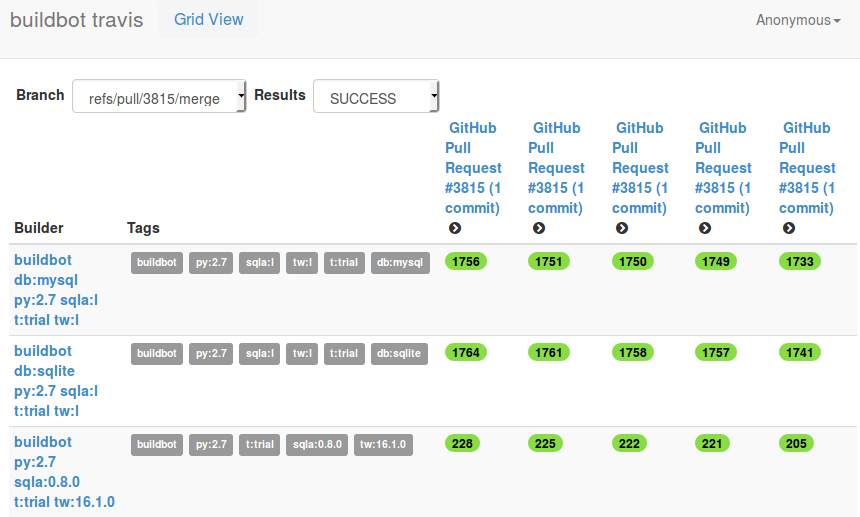
\includegraphics[clip,width=15cm]{grid_view}
\par\end{centering}
\caption{Sample grid view\label{fig:Sample-grid-view}}
\end{figure}

\subsection{Waterfall view}

Waterfall shows the whole activity in a vertical timeline.
Builds are represented with boxes whose height vary according to their
duration. Builds are sorted by builders in the horizontal axes, which
allow you to see how builders are scheduled together.\citep{www-waterfall}

\begin{figure}[H]
\begin{centering}
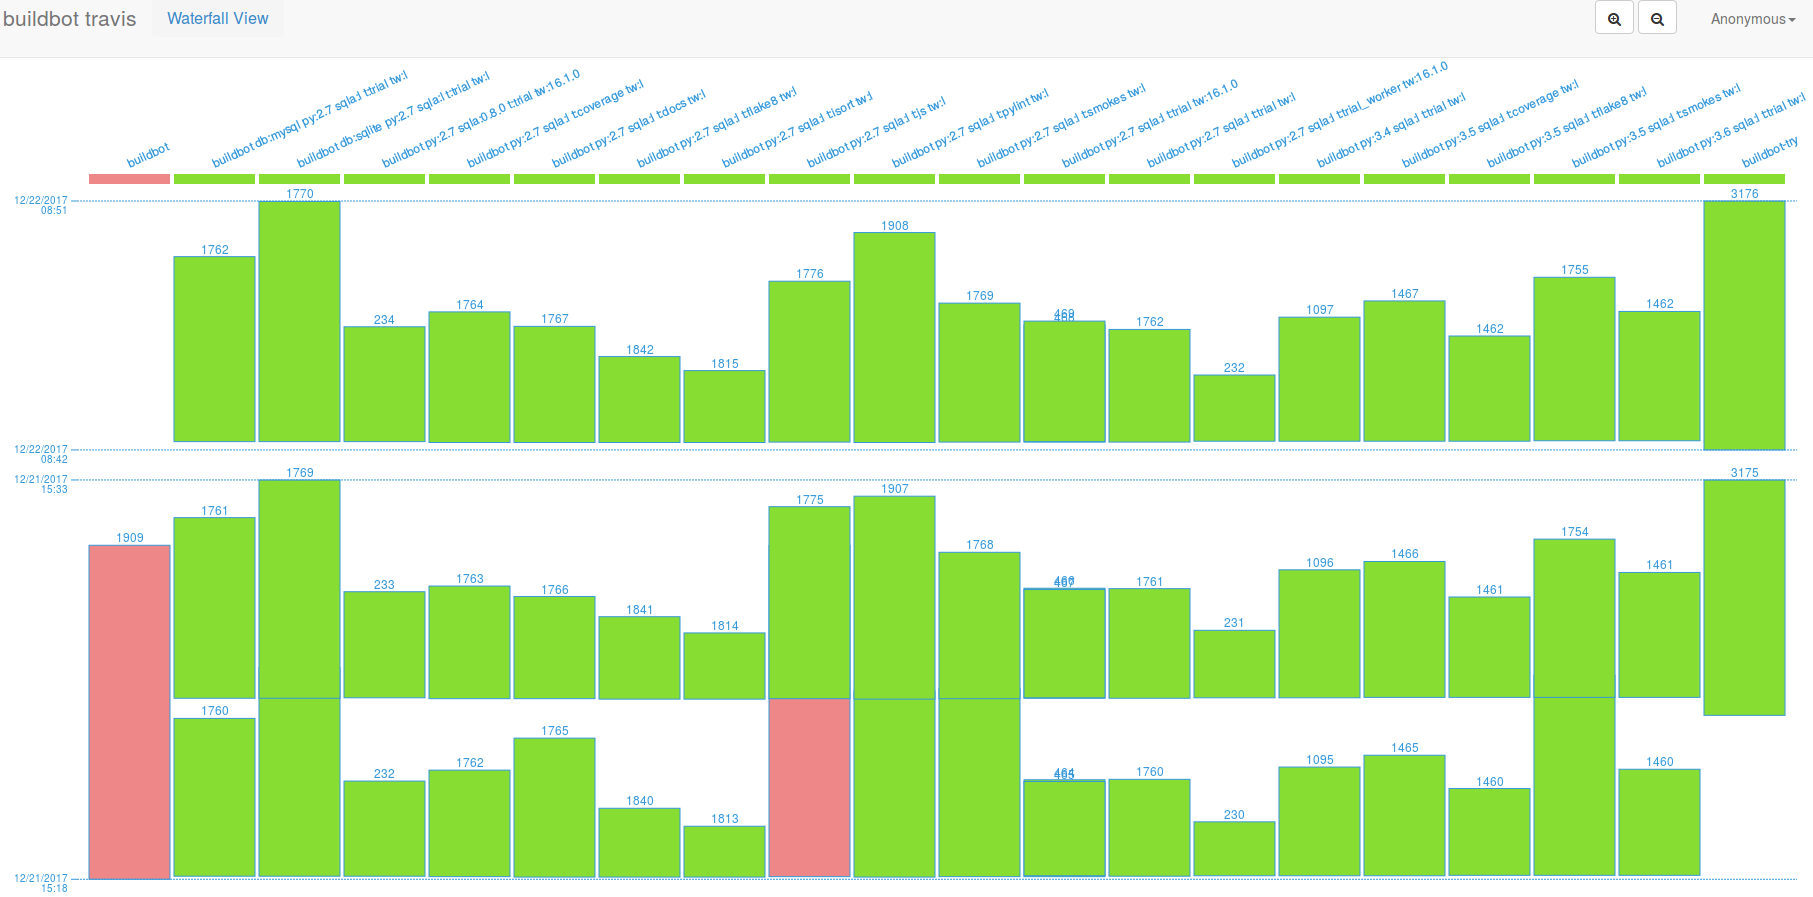
\includegraphics[clip,width=15cm]{waterfall_view}
\par\end{centering}
\caption{Sample waterfall view\label{fig:Sample-waterfall-view}}
\end{figure}

\subsection{Console view}

Console view shows the whole buildbot activity arranged by changes
as discovered by Change Sources vertically and builders horizontally.
If a builder has no build in the current time range, it will not be
displayed.

Console view will also group the builders by tags. When there are
several tags defined per builders, it will first group the builders
by the tag that is defined for most builders. Then given those builders,
it will group them again in another tag cluster.\citep{www-console}

\begin{figure}[H]
\begin{centering}
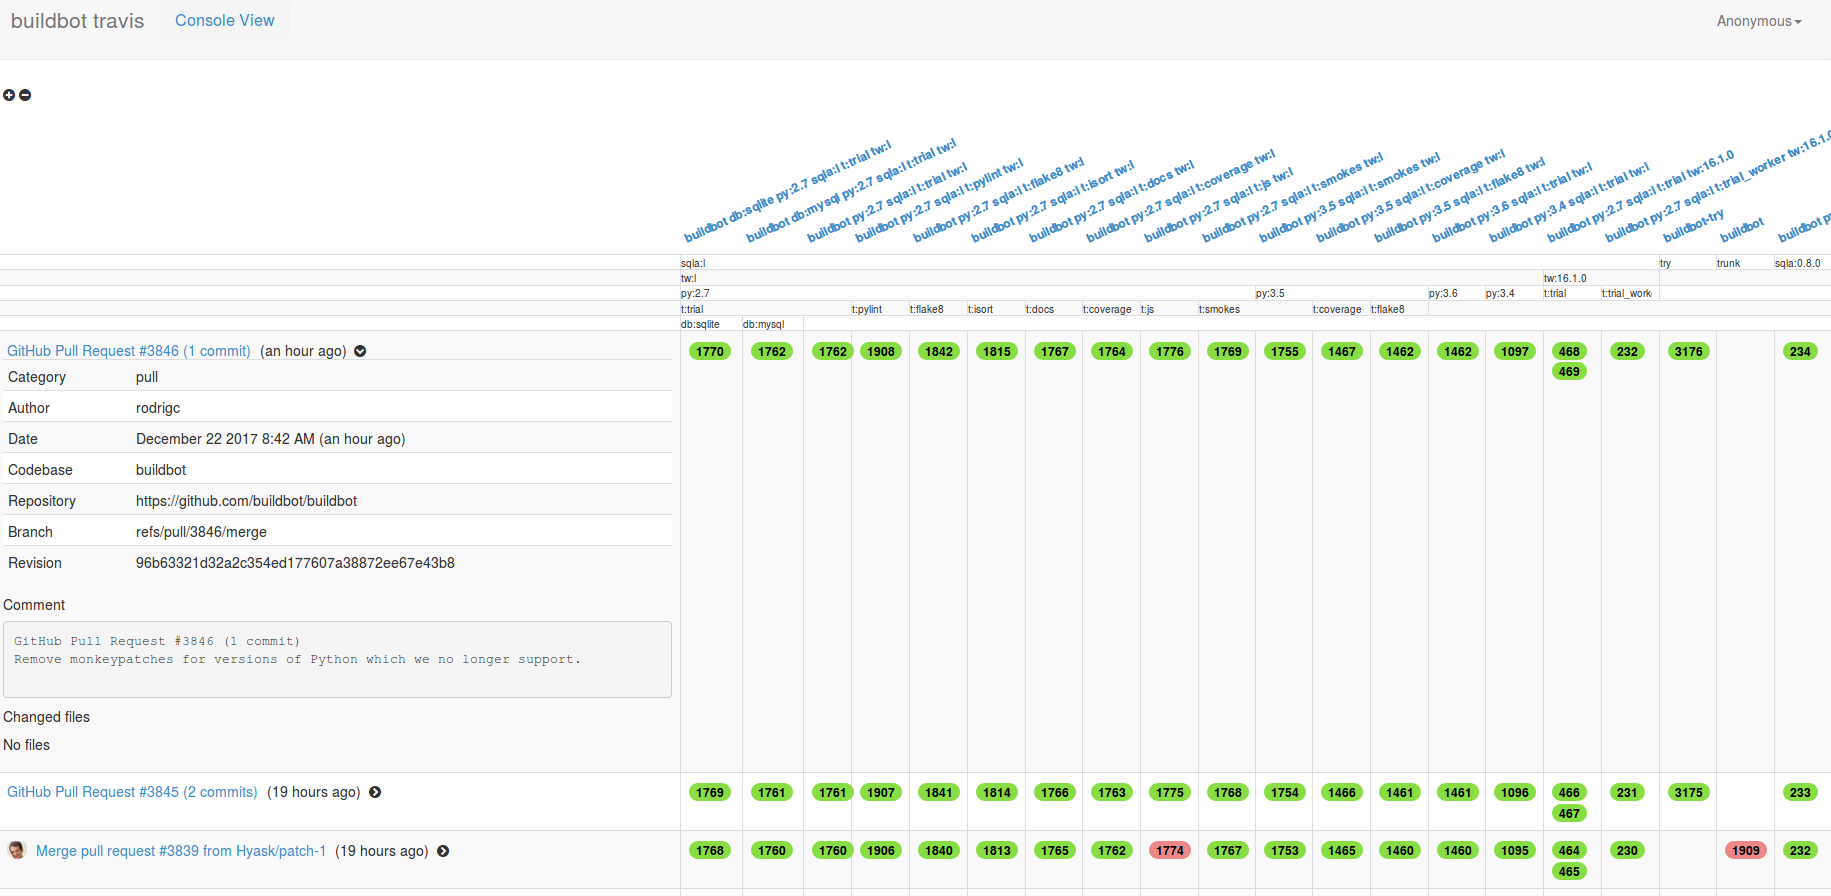
\includegraphics[clip,width=15cm]{console_view}
\par\end{centering}
\caption{Sample console view\label{fig:Sample-console-view}}
\end{figure}

\subsection{Settings}

The settings page provides some option tweaking accessible for the
user, and more important configuration options for logged in administrators.
These settings can be extended in the buildbot Angular app.

\begin{figure}[H]
\begin{centering}
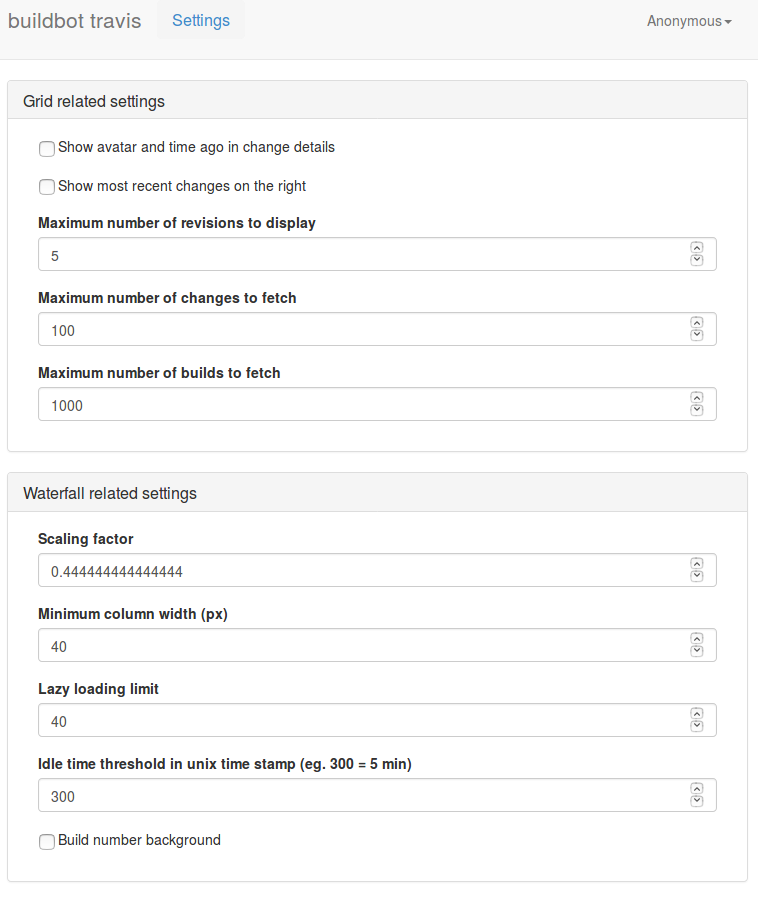
\includegraphics[clip,width=15cm]{bb_settings}
\par\end{centering}
\caption{Sample settings menu\label{fig:Sample-settings-menu}}
\end{figure}

\chapter{Custom implementations}

\section{Backend componentization}

By default, the Buildbot master configuration resides in the \texttt{master.cfg}
file in the buildmaster's base directory. A sample file is automatically
installed when a new master is created.

The config file is written in Python and it defines a dictionary named
\texttt{BuildmasterConfig}, with a number of keys that are specially
treated. Being a pythonic configuration, we can benefit from the features
of the programming language, such as componentization of the configuration
parts into modules. This comes in handy when we are dealing with large
configurations. At first the \texttt{master.cfg} file seems suitable,
but as we add more builders and workers, we need to keep the code
readable, thus we split \texttt{master.cfg} into multiple modules.

The figure below illustrates this componentization for the Nokia Buildbot
project, which has 4 projects running on the same master (CAS, INCT,
FRI, DEM), each of them having an arbitrary number of builders (\texttt{builders}
subfolder) and a specific web dashboard (\texttt{dashboard} subfolder).

Some of the build steps have log outputs that do not match Buildbot's
default parsers, so custom logparsers have been implemented (\texttt{builders/steps}
subfolder). 

Custom notifiers have the purpose of informing the user/admin about
vital build or system information, the current implemented one uses
LDAP to query the active directory in order to find the e-mail address
of an user (\texttt{notifier} subfolder). 

As the project increases in size, metrics become necessary. We use
Prometheus to keep track of information, and Grafana to crunch it
and present it in an user-friendly way (\texttt{reporters} subfolder).

All of these components could be worked into the \texttt{master.cfg}
file, but the result would be an approx. 2300 line configuration file
that encompasses each category, making code modifications and additions
more prone to errors and most certainly a chore to go through.

\begin{figure}[H]
\begin{centering}
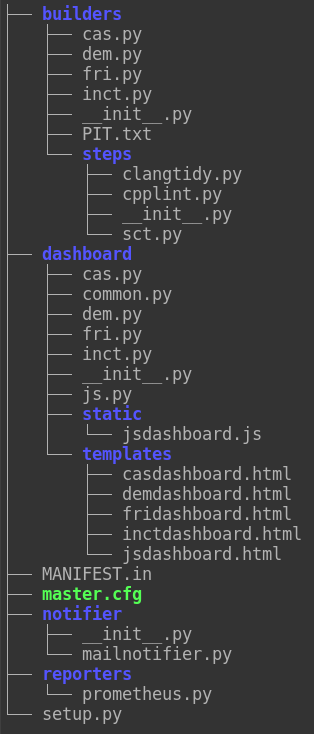
\includegraphics[scale=0.5]{config_tree}
\par\end{centering}
\caption{Sample configuration componentization}

\end{figure}

\subsection{Email look-up using LDAP}

Making users aware of their build status and results is an important
part of the CI process. To keep user input to a minimum, we can figure
out their e-mail address from their Linux username. For this purpose,
we use Python's LDAP (Lightweight Directory Access Protocol) module
to search through the active directory for the user's information.

To send e-mails to users, Buildbot provides a \texttt{MailNotifier}
reporter that does most of the job. This is a basic example:

\begin{listing}[H]
    \caption{\texttt{mailnotifier\_default.py}}
    \inputminted[breaklines]{python}{code/mailnotifier_default.py}
\end{listing}

Concerning our use case, we need to configure a proper \texttt{lookup}
function. For builds triggered by VCS commits, this is automatically
managed by adding the e-mail addresses of the committers. However,
try builds do not provide the e-mail parameter, so it has to be figured
out using the user's Unix username.
\begin{figure}[H]
\begin{centering}
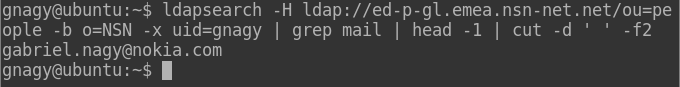
\includegraphics[width=15cm]{ldap_bash}
\par\end{centering}
\caption{Using \texttt{ldapsearch} to get the e-mail address from the Active
Directory}
\end{figure}

For Buildbot integration, we have to implement an \texttt{IEmailLookup}
interface that is provided by Buildbot. This interface has a \texttt{getAddress}
method that turns an username string into a valid e-mail address.\citep{email-lookup}

To implement the interface, we need to adapt the \texttt{ldapsearch}
to Python code:

\begin{listing}[H]
    \caption{\texttt{IEmailLookup.py}}
    \inputminted[breaklines]{python}{code/iemaillookup.py}
\end{listing}

As shown in the code, the class takes an optional argument, \texttt{emailsMap},
which is a dictionary of username and e-mail key/value pairs. This
is usually done to avoid querying the Active Directory for an user
that has used the system before.

Finally, to deploy this interface, we import it in the master configuration
file, and we adjust our \texttt{MailNotifier} reporter accordingly,
also adding a HTML template as desired:

\begin{listing}[H]
    \caption{\texttt{mailnotifier\_extended.py}}
    \inputminted[breaklines]{python}{code/mailnotifier_extended.py}
\end{listing}

Now, each time user-triggered builds on builders with the \texttt{cas}
tag are completed, the user receives an e-mail with the status of
his build. If the user submitted a patchfile, it is also included
in the e-mail.
\begin{figure}[H]
\begin{centering}
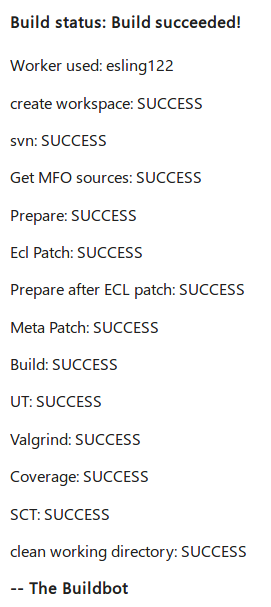
\includegraphics[scale=0.5]{mail_contents}
\par\end{centering}
\caption{Contents of the e-mail sent by Buildbot}
\end{figure}

\subsection{Log parsing}

Buildbot provides a number of parsers for commonly used commands such
as compilers (cmake, make, visual c++...) and tests (cppcheck, make
test, trial...). However, there are special cases that do not fit
the default parsers and custom ones have to be implemented.\citep{concepts-logobservers}

As it will be used in other sections, we will implement a simple parser
for the \texttt{clang-tidy} command. We begin by creating a new class
that inherits the default \texttt{ShellCommand}. We provide the class
with a \texttt{logConsumer} function that incrementally gets every
line of the command's output, and we feed the lines to the \texttt{gatherTestStatistics}
function that parses the lines. We use Python's regular expressions
module to search for the desired content.

\begin{listing}[H]
    \caption{\texttt{clangtidy.py}}
    \inputminted[breaklines]{python}{code/clangtidy_1.py}
\end{listing}

The \texttt{\_\_init\_\_} function initializes our new \texttt{ShellCommand},
adding a log observer to the \texttt{stdio} output, and providing
initial fields for possible errors and warnings.

\begin{listing}[H]
    \caption{\texttt{clangtidy.py}}
    \inputminted[breaklines]{python}{code/clangtidy_2.py}
\end{listing}

The command is mostly done as we successfully parsed its output. However,
it must be evaluated in order to set a status after the step is finished.
The evaluation is straightforward, if we have something in the \texttt{errors}
field, we mark the step as failed, if we have \texttt{warnings} and
no \texttt{errors}, we mark the step as having warnings (the build
will not stop).

\begin{listing}[H]
    \caption{\texttt{clangtidy.py}}
    \inputminted[breaklines]{python}{code/clangtidy_3.py}
\end{listing}

We successfully implemented our parser, however the user does not
know the error/warning count until he opens the log. To fix that,
we can update the step's description with the count.

\begin{listing}[H]
    \caption{\texttt{clangtidy.py}}
    \inputminted[breaklines]{python}{code/clangtidy_4.py}
\end{listing}

We now have a fully working \texttt{clang-tidy} command parser. It
is a good practice to write unit tests for our code, so we make a
generic test suite:

\begin{listing}[H]
    \caption{\texttt{clangtidy\_test.py}}
    \inputminted[breaklines]{python}{code/clangtidy_test.py}
\end{listing}

All that remains to do is to import this class into the configuration
file, and create the step using \texttt{steps.ClangTidy} instead of
\texttt{steps.ShellCommand}.

Buildbot now correctly processes the output and updates the result
accordingly:
\begin{figure}[H]
\begin{centering}
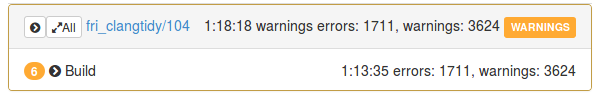
\includegraphics[width=15cm]{clangtidy_summary}
\par\end{centering}
\caption{clang-tidy command output}
\end{figure}

\subsection{Preferential build steps}

In our use cases, there is the possibility of patching more than one
component in a build. By default, Buildbot executes all commands until
failed.

\texttt{BuildStep}s are usually specified in the buildmaster\textquoteright s
configuration file, in a list that goes into the \texttt{BuildFactory}.
The \texttt{BuildStep} instances in this list are used as templates
to construct new independent copies for each build (so that state
can be kept on the \texttt{BuildStep} in one build without affecting
a later build). Each \texttt{BuildFactory} can be created with a list
of steps, or the factory can be created empty and then steps added
to it using the \texttt{addStep} method:

\begin{listing}[H]
    \caption{\texttt{simple\_factory.py}}
    \inputminted[breaklines]{python}{code/simple_factory.py}
\end{listing}

However, we would like to execute only certain commands, depending
on the status of the previous commands. To accomplish that, we need
to know that Buildbot steps finish with a status described by one
of four values defined in \texttt{buildbot.status.builder}: \texttt{SUCCESS},
\texttt{WARNINGS}, \texttt{FAILURE} or \texttt{SKIPPED}.\citep{concepts-buildsteps}

Let's say that we have a builder that checks out a source, runs a
linter and builds the code only if the lint step had no errors, then
cleans up the build folder. An example for this use case can be seen
below:

\begin{listing}[H]
    \caption{\texttt{preferential\_factory.py}}
    \inputminted[breaklines]{python}{code/preferential_factory.py}
\end{listing}

To skip a step, Buildbot provides us with the \texttt{doStepIf} parameter
for a \texttt{ShellCommand} . The value is set to a lambda function
that returns \texttt{True} only if the previous step's result is \texttt{FAILURE}.

\texttt{step.build.executedSteps} is a list of the executed steps
including the one that is running when the list is queried. We get
the result of the \texttt{clang-tidy} command by selecting the second
to last executed step. In Python this is easily done by going backwards
on the list, providing it with a negative value (\texttt{{[}-2{]}}).

At the end, we want to clean the workspace so it does not interfere
with future builds. By default, Buildbot stops a build when a step
fails. To override that, we provide the \texttt{rm -rf} command with
the \texttt{alwaysRun} parameter.

\section{Web interface development}

While Buildbot's default web views (console, grid, waterfall) may
be useful for some users, the real advantage lies in their customizability.
We will build the same custom dashboard twice, once with Flask/WSGI,
and once with Angular. At the end, we will compare and contrast the
two approaches.

\subsection{Flask/WSGI dashboards}

The simpler way, for most Python developers, is to use the \texttt{buildbot\_wsgi\_dashboards
}plugin to write a server side generated dashboard and integrate it
in the UI.

The plugin is compatible with any WSGI web framework, we will use
Flask as it is one of the more popular ones. A \texttt{/index.html}
route needs to be implemented, which will render the code representing
the dashboard. The application framework runs in a thread outside
of Twisted and it provides a synchronous wrapper for accessing the
Data API. The HTML output is ran inside the Angular application, using
its CSS and some of the directives defined by the Buildbot UI. It
also has full access to the application JS context.\citep{buildbot-flask}

For our custom dashboard, we need to be able to filter by tag, and
to show both poller-triggered builds and manually triggered builds.
Our end result will look similar to this figure:
\begin{figure}[H]
\begin{centering}
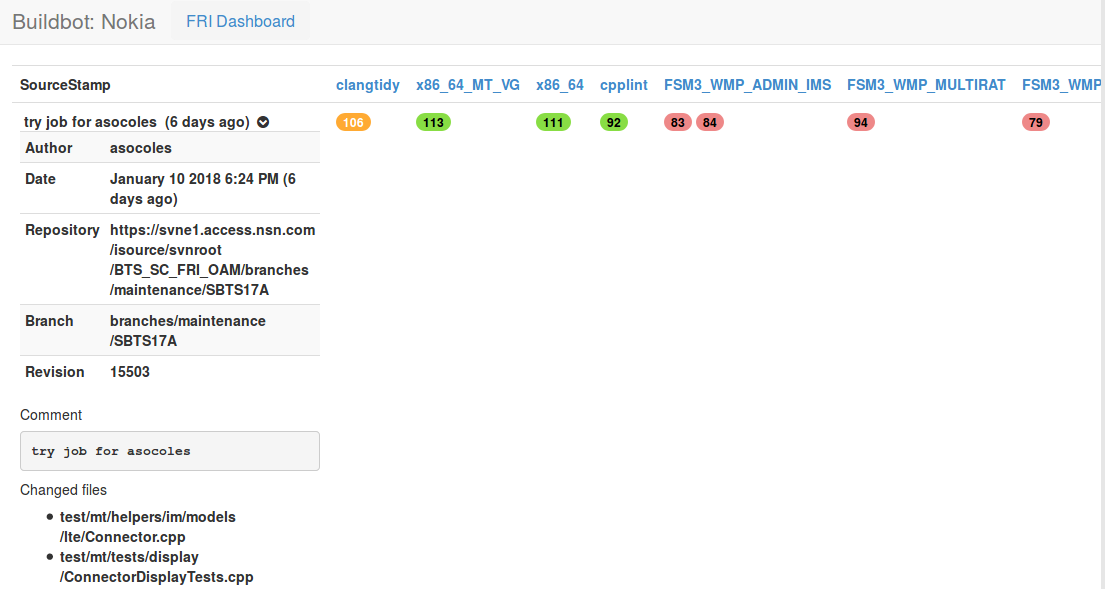
\includegraphics[width=15cm]{dashboard_build}
\par\end{centering}
\caption{Custom dashboard result}
\end{figure}

We begin by creating the logic for the dashboard. First we create
the helper functions for obtaining the changed file list and the fake
change creator, since Buildbot doesn't generate one when triggering
a manual build:

\begin{listing}[H]
    \caption{\texttt{helper\_functions.py}}
    \inputminted[breaklines]{python}{code/helper_flask.py}
\end{listing}

We will use of this data when filling in the template fields. By making
use of Buildbot's Data API we obtain information about the builders
and buildsets that we want to display:

\begin{listing}[H]
    \caption{\texttt{flask\_dashboard.py}}
    \inputminted[breaklines]{python}{code/flask_1.py}
\end{listing}

Next, we iterate through the buildsets, keeping the ones that interest
us, and saving the information that we want to show in the template:

\begin{listing}[H]
    \caption{\texttt{flask\_dashboard.py}}
    \inputminted[breaklines]{python}{code/flask_2.py}
\end{listing}

At the end we return the template with our parsed content, the builders
and a dictionary of all the related data we want to show:

\begin{listing}[H]
    \caption{\texttt{flask\_dashboard.py}}
    \inputminted[breaklines]{python}{code/flask_3.py}
\end{listing}

To keep the page small, we remove the bloat by minifying our HTML
response. This can be easily done in Flask with the help of the \texttt{@after\_request}
decorator:

\begin{listing}[H]
    \caption{\texttt{flask\_dashboard.py}}
    \inputminted[breaklines]{python}{code/flask_4.py}
\end{listing}

For the HTML part, we generate a simple table, filling it out with
the data returned by our Flask file:

\begin{listing}[H]
    \caption{\texttt{flask\_template.html}}
    \inputminted[breaklines]{html}{code/flask_template.html}
\end{listing}

The only thing left to do is to load our dashboard in the \texttt{master.cfg}
file. We do this by importing our Flask file and appending to the
\texttt{c{[}'www'{]}{[}'plugins'{]}{[}'wsgi\_dashboards'{]}} key:

\begin{listing}[H]
    \caption{\texttt{master.cfg}}
    \inputminted[breaklines]{python}{code/flask_master.py}
\end{listing}

After we restart/reconfig our Buildbot, our new dashboard can be seen
in the sidebar:
\begin{figure}[H]
\begin{centering}
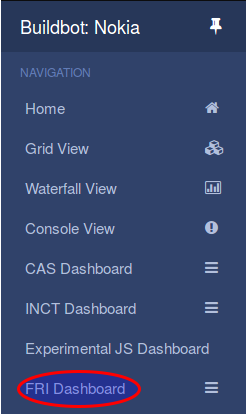
\includegraphics[scale=0.8]{buildbot_sidebar}
\par\end{centering}
\caption{Newly modified sidebar}
\end{figure}

\subsection{Angular dashboards}

Though easy to implement and familiar to Python developers, the Flask
dashboard is not efficient for long term use, since it is not asynchronously
updated when builds are added, and the whole page has to be reloaded,
making this a very time and resource consuming activity.

The right solution would be to follow the approach of \emph{Console}
and \emph{Waterfall view} and create these dashboards as Buildbot
plugins using Angular. By choosing this approach, we benefit from
real-time loading with AJAX, reducing our load by a large margin.
For developers unfamiliar with Node.js and its practices, this approach
may seem unfriendly. Fortunately, the developers have put up a ``quick-start
guide'' for Angular live coding.\citep{buildbot-angular} In short,
one has to locally build the frontend of Buildbot, scaffold a dashboard
template and install a browser plugin in order to benefit from live
reloading when the code changes.

Using CoffeeScript and Jade, we recreate the dashboard logic previously
used with Flask. After we set up our environment,\citep{buildbot-www-base-app}
we can begin coding.

Because the scaffold sets up the project for us, we only need to concern
ourselves with 4 files:
\begin{itemize}
\item \texttt{main.module.coffee}, which registers our state and module
\item \texttt{main.module.spec.coffee}, where we provide modules for use
in the controller file
\item \texttt{dashboard.controller.coffee}, which provides the logic for
our dashboard
\item \texttt{dashboard.tpl.jade}, which provides the template for the dashboard
\end{itemize}
We start by ``translating'' our Python/Flask logic into CoffeeScript:

\begin{listing}[H]
    \caption{\texttt{dashboard.controller.coffee}}
    \inputminted[breaklines]{coffee}{code/dashboard_constructor.txt}
\end{listing}

At first, we prepare our global variables and we get all buildsets
from the past 7 days using the Buildbot Data API. To benefit from
the colored build dots (as seen in the Flask dashboard), we need to
include \texttt{resultsService} in the constructor. \texttt{dataService}
provides us with the connection to the data API, and \texttt{@\$uibModal}
helps us create modal popups when builds are clicked. Next, we parse
the buildsets for the needed information, also taking into account
\emph{pending} buildsets/buildrequests:
\begin{code}
\captionof{listing}{\texttt{dashboard.controller.coffee}}
\begin{minted}[breaklines]{coffee}
  onChangeBuildsets: =>
    if not (@buildsets.$resolved and @buildsets.length > 0)
      return

    getChangeFromBbSourceStamp = (sourcestampdetails) ->
      fakeChange = {
        "revision": sourcestampdetails['revision'],
        "when_timestamp": sourcestampdetails['created_at'],
        "codebase": sourcestampdetails['codebase'],
        "repository": sourcestampdetails['repository'],
        "branch": sourcestampdetails['branch'],
      }
      if sourcestampdetails.hasOwnProperty('patch') and sourcestampdetails['patch']
        fakeChange["author"] = sourcestampdetails['patch']['author']
        fakeChange["comments"] = sourcestampdetails['patch']['comment']
      return fakeChange

    for buildset in @buildsets
      sourcestamps = buildset['sourcestamps']
      if sourcestamps.length != 1
        console.log("Unexpected sourcestamps for buildset " + buildset['bsid'])
      sourcestamp = sourcestamps[0]
      ssid = sourcestamp['ssid']
      if not @sourcestampsMap.hasOwnProperty(ssid)
        @sourcestampsMap[ssid] = {
          change: getChangeFromBbSourceStamp(sourcestamp),
          buildsets : []
        }
      @sourcestampsMap[ssid]['buildsets'].push(buildset['bsid'])
      @buildrequestsGetMap[buildset['bsid']] = @data.getBuildrequests(buildsetid: buildset['bsid'])
      @buildrequestsGetMap[buildset['bsid']].onChange = @onChangeBuildrequests

  onChangeBuildrequests: =>
    for id, buildreq of @buildrequestsGetMap
      if not buildreq.$resolved
        return

    for buildsetid, buildrequests of @buildrequestsGetMap
      @buildsetsMap[buildsetid] = {}
      @buildsetsMap[buildsetid]['pendingBuildrequests'] = {}
      @buildsetsMap[buildsetid]['claimedBuildrequests'] = {}

      for buildrequest in buildrequests
        buildrequestid = buildrequest['buildrequestid']

        if buildrequest["claimed"]
          @buildsGetMap[buildrequestid] = @data.getBuilds(buildrequestid: buildrequestid)
          @buildsGetMap[buildrequestid].onChange = @onChangeBuild
          @buildsetsMap[buildsetid]['claimedBuildrequests'][buildrequestid] = buildrequest
        else
          @buildsetsMap[buildsetid]['pendingBuildrequests'][buildrequestid] = buildrequest

  onChangeBuild: =>
    for id, bld of @buildsGetMap
      if not bld.$resolved
        return
    for buildrequestid, builds of @buildsGetMap
      @buildrequestsMap[buildrequestid] = {}
      for build in builds
        @buildrequestsMap[buildrequestid][build['buildid']] = build
    @generateBuildsMap()
\end{minted}
\end{code}

For our modal view, we have the selectBuild\texttt{ }function to redirect
the user to the modal template when clicked:

\begin{listing}[H]
    \caption{\texttt{dashboard.controller.coffee}}
    \inputminted[breaklines]{coffee}{code/modal_dashboard.txt}
\end{listing}

This sums up our controller. In the spec file, we need to tell the
application to provide us with our additional services (result and
modal):

\begin{listing}[H]
    \caption{\texttt{main.module.spec.coffee}}
    \inputminted[breaklines]{coffee}{code/module_spec.txt}
\end{listing}

The template needs little tinkering, but looks better than the Flask
one because we kept all the dashboard logic in the controller:

\begin{listing}[H]
    \caption{\texttt{dashboard.tpl.jade}}
    \inputminted[breaklines]{jade}{code/dashboard_template.txt}
\end{listing}

Our dashboard is now complete and the modal popup looks like this:
\begin{figure}[H]
\begin{centering}
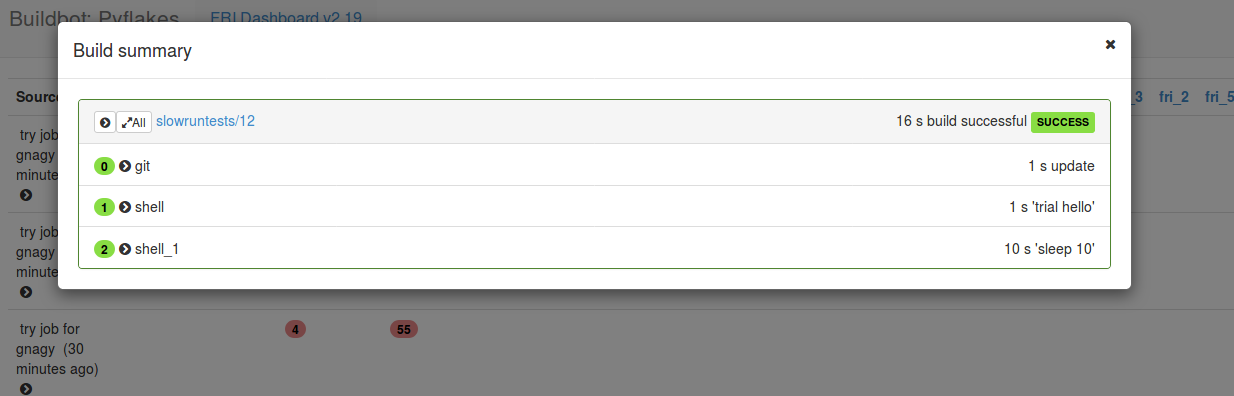
\includegraphics[width=15cm]{dashboard_modal}
\par\end{centering}
\caption{Modal view when clicking on a build sticker}
\end{figure}

\section{User scripts}

All is well and good with our dashboards, but we need a way to trigger
our builds, apart from our regular version control poller. For that,
the internal \texttt{buildbot try} command can help us. However, an
usual try command looks like this: \texttt{buildbot try -{}-who=\char`\"{}gnagy\char`\"{}
-{}-connect=pb -{}-vc=git -{}-topdir=. -{}-master=localhost:8031 \newline-{}-username=\char`\"{}change\char`\"{}
-{}-passwd=\char`\"{}changepw\char`\"{} -{}-branch=master -{}-builder=slowruntests
-{}-builder=runtests -{}-comment=\char`\"{}try job for gnagy\char`\"{}
\newline-{}-repository=https://github.com/buildbot/hello-world.git}.

This command assumes the following: 
\begin{itemize}
\item we are in the \texttt{hello-world} Git repository and we have uncommitted
changes in the code
\item \texttt{pb} is the protocol we use to transfer our data
\item \texttt{change} and \texttt{changepw} are our login credentials
\item \texttt{localhost:8031} is the port on which our try \emph{scheduler}
listens
\item \texttt{runtests} and \texttt{slowruntests} are the builders which
we want to trigger
\item \texttt{who} is our name and \texttt{comment} is an optional message
that we may want to specify
\item \texttt{git} is the version control system that we use in the repository
\item \texttt{https://github.com/buildbot/hello-world.git} is the repository
URL
\end{itemize}
Next, \texttt{buildbot try} automatically generates a patch containing
our uncommitted code and sends it to the try scheduler active on the
master, triggering builds on our specified builders. The build commands
execute as usual, with the patch automatically applying after the
repository is checked out.

For a developer who just wants to test his code, almost if not all
of this information is useless. It should be enough for him to type
a one-word command such as \texttt{try\_diff}. All of the required
information can be automatically generated and completed. For that,
we devise a Python script with the role to simplify the cluttered
syntax of \texttt{buildbot try}.

Basically, we need to create a wrapper around the \texttt{try} script,
automatically completing all fields with default values, but we also need
to let the users override them if needed. Assuming we prepared the script
for a certain project that the developer works on, we do not need anything more 
except for him to run the script from his working directory (provided it has uncommitted changes).

We begin by hardcoding the dictionary containing the configuration options, which are mandatory and should not be changed by the user.
We also add a shebang line to let the system know that the file is to be always executed with Python, to simplify usage.
\begin{code}
\captionof{listing}{\texttt{try\_diff} - configuration}
\begin{minted}[breaklines]{python}
#!/usr/bin/env python
configuration = {
    "repo_addr": "https://github.com/buildbot/hello-world.git",
    "repo_type": "git",
    "try_scheduler_address": "localhost:8031",
    "username": "change",
    "password": "changepw"
}
\end{minted}
\end{code}

Next, we define the two main functions of the script, which are:
\begin{itemize}
\item \texttt{compose\_patch\_cmd} - the function that translates our properties and parameters as buildbot try parameters, and returns the command to be called
\item \texttt{trigger\_buildbot} - the function that actually executes the buildbot try command
\end{itemize}

To improve our script, we add \texttt{verbose} and \texttt{dryrun} options, in case the user wants to see how the command is run, or just to simulate the command.
\begin{code}
\captionof{listing}{\texttt{try\_diff} - functions}
\begin{minted}[breaklines]{python}
def compose_patch_cmd(who, repo_type, scheduler, login, password, project_repo, branch, builders, comments, patch, filelist):
    change_cmd = "buildbot try "
    change_cmd += '--who="%s" ' % who
    change_cmd += "--connect=pb "
    change_cmd += "--vc=%s " % repo_type
    change_cmd += "--topdir=. "
    change_cmd += "--master=%s " % scheduler
    change_cmd += '--username="%s" ' % login
    change_cmd += '--passwd="%s" ' % password
    change_cmd += "--repository=%s " % project_repo
    change_cmd += "--branch=%s " % branch
    change_cmd += "--project=test_proj "
    if patch:
        assert(os.path.exists(patch))
        change_cmd += "--diff=%s " % patch
    if builders:
        for builder in builders:
            change_cmd += "--builder='%s' " % builder
    change_cmd += '--comment="%s" ' % comments
    change_cmd += '--property=author=%s ' % who
    change_cmd += '--property=comment="%s" ' % comments
    change_cmd += '--property=filelist="%s" ' % filelist

    return change_cmd


def trigger_buildbot(who, configuration, branch, comments="", patch=None, builders=[], filelist=None, dryrun=False, verbose=False):
    if patch:
        command = compose_patch_cmd(who,
                                    configuration["repo_type"],
                                 configuration["try_scheduler_address"],
                                    configuration["username"],
                                    configuration["password"],
                                    configuration["repo_addr"],
                                    branch,
                                    builders,
                                    comments,
                                    patch,
                                    filelist)

    if verbose:
        print('\n' + command)

    if not dryrun:
        subprocess.check_call(command, shell=True)
\end{minted}
\end{code}

Next, we create our argument parser, which we fill up by default,
letting the user override the values if needed.

\begin{code}
\captionof{listing}{\texttt{try\_diff} - parser}
\begin{minted}[breaklines]{python}
default_patch = 'patch.txt'
default_branch = subprocess.check_output(['git', 'rev-parse', '--abbrev-ref', 'HEAD'])
diff_command = "git diff > patch.txt"

parser = argparse.ArgumentParser(description='Script for triggering buildbot try build', formatter_class=RawTextHelpFormatter)

parser.add_argument('-n', '--dry-run', dest='dryrun', action='store_true', required=False, default=False, help="don't trigger anything; exit after printing command")
parser.add_argument('-v', '--verbose', dest='verbose', action='store_true', required=False, default=False, help="increase verbosity")
parser.add_argument('-a', '--author', dest='author', type=str, required=False, default=os.getenv('USER', 'ninja_trigger'), help="any author string")
parser.add_argument('-c', '--comment', dest='comment', type=str, required=False, default="try job for " + os.getenv('USER'), help="any comment string")
parser.add_argument('-B', '--builder', dest='builder', type=str, required=False, action='append', default=None, help="builder name, can be specified multiple times, e.g. -B runtests0 -B slowruntests\n If no builder is specified all builders are triggered.")
parser.add_argument('-p', '--patch', dest='patchfile', type=str, required=False, default=default_patch, help="generated patch file (if applicable), e.g.\n  git diff > patchfile.txt\nIf no patch is specified, git diff will be run automatically.")
parser.add_argument('-b', '--branch', dest='branch', type=str, required=False, default=default_branch, help="branch name, e.g. master\n")
args = parser.parse_args()
\end{minted}
\end{code}

So, the bulk of the script has been established. We now 


\section{Capturing metrics}

buildbot metrics + Prometheus \textbackslash{}w alertmanager + grafana

\section{Extending the source code}

extending buildbot source to allow multiple patchfiles and more API
entrypoints maybe?

\chapter{Conclusion}
\begin{thebibliography}{99}
\bibitem{python-usage}{McConnell, Steve, Code Complete, Microsoft
Press, 2009, p. 100} 

\bibitem{python-about}{About Python, URL: \url{https://www.python.org/about/}} 

\bibitem{python-popularity}{TIOBE Index for November 2017, URL:
\url{https://www.tiobe.com/tiobe-index/}} 

\bibitem{python-empirical-comparison}{Prechelt, Lutz, An empirical
comparison of C, C++, Java, Perl, Python, Rexx, and TCL, Fakult\"{a}t
f\"{u}r Informatik, Universit\"{a}t Karlsruhe, 2000} 

\bibitem{twisted-intro}{McKellar, J. and Fettig, A., Twisted Network
Programming Essentials, O'Reilly Media, 2013, p. xiii}

\bibitem{twisted-example}{McKellar, J. and Fettig, A., Twisted Network
Programming Essentials, O'Reilly Media, 2013, p. 11}

\bibitem{twisted-ideas}{Twisted Framework: Core ideas, URL: \url{https://en.wikipedia.org/w/index.php?title=Twisted_(software)&oldid=808304626 }}

\bibitem{sqlite-apress}{Owens, Michael, The Definitive Guide to
SQLite, Apress, 2014, p. 133} 

\bibitem{sqlite-deployed}{Most Widely Deployed SQL Database Engine,
URL: \url{https://sqlite.org/mostdeployed.html}} 

\bibitem{buildbot-introduction}{Introduction - Buildbot latest documentation,
URL: \url{http://docs.buildbot.net/current/manual/introduction.html}} 

\bibitem{buildbot-database}{Database - Buildbot latest documentation,
URL: \url{http://docs.buildbot.net/latest/developer/database.html}} 

\bibitem{buildbot-cfg}{Global Configuration - Buildbot latest documentation,
URL: \url{http://docs.buildbot.net/latest/manual/cfg-global.html}} 

\bibitem{angular-architecture}{Angular - Architecture Overview,
URL: \url{https://angular.io/guide/architecture}} 

\bibitem{angular-how-it-works}{AngularJS - Wikipedia, URL: \url{https://en.wikipedia.org/w/index.php?title=AngularJS&oldid=812169171}} 

\bibitem{angular-introduction}{AngularJS: Developer Guide: Introduction,
URL: \url{https://docs.angularjs.org/guide/introduction}} 

\bibitem{node-whatis}{What is Node.js? - Definition from WhatIs.com,
URL: \url{http://whatis.techtarget.com/definition/Nodejs}} 

\bibitem{npm-guide}{A Beginner's Guide to npm - the Node Package
Manager, URL: \url{https://www.sitepoint.com/beginners-guide-node-package-manager}} 

\bibitem{npm-ampersand}{Ampersand.js - Learn, URL: \url{https://ampersandjs.com/learn/npm-browserify-and-modules}} 

\bibitem{npm-security}{Ojamaa, Andres; Duuna, Karl, Assessing the
Security of Node.js Platform, URL: \url{http://ieeexplore.ieee.org/stamp/stamp.jsp?tp=&arnumber=6470829}}

\bibitem{npm-understanding}{Understanding npm, URL: \url{https://unpm.nodesource.com}}

\bibitem{npm-conduct}{npm Code of Conduct: acceptable package content,
URL: \url{https://www.npmjs.com/policies/conduct\#acceptable-package-content}}

\bibitem{npm-stat}{npm-stat: download statistics for NPM packages,
URL: \url{https://npm-stat.com}}

\bibitem{npm-manage}{How To Use npm to Manage Node.js Packages on
a Linux Server, URL: \url{https://www.digitalocean.com/community/tutorials/how-to-use-npm-to-manage-node-js-packages-on-a-linux-server}}

\bibitem{npm-install}{npm-install, URL: \url{https://docs.npmjs.com/cli/install}}

\bibitem{npm-semver}{semver, URL: \url{https://docs.npmjs.com/misc/semver}}

\bibitem{npm-version}{npm-version, URL: \url{https://docs.npmjs.com/cli/version}}

\bibitem{npm-yarn}{The npm Blog - Hello, Yarn!, URL: \url{http://blog.npmjs.org/post/151660845210/hello-yarn}}

\bibitem{npm-facebook}{Yarn: A new package manager for JavaScript
\textbar{} Engineering Blog \textbar{} Facebook Code, URL: \url{https://code.facebook.com/posts/1840075619545360/yarn-a-new-package-manager-for-javascript}}

\bibitem{gulp-whatis}{Mao, Jed; Schmitt, Maximilian; Stryjewski,
Tomasz; Country Holt, Cary; Lubelski, Wiliam, Developing a Gulp Edge
(1st ed.), Bleeding Edge Press, 2014} 

\bibitem{gulp-pipelines}{substack/stream-handbook: how to write
note programs with streams, URL: \url{https://github.com/substack/stream-handbook}}

\bibitem{gulp-readme}{gulpjs/gulp: Writing a plugin, URL: \url{https://github.com/gulpjs/gulp/blob/master/docs/writing-a-plugin/README.md}}

\bibitem{gulp-building}{Building With Gulp - Smashing Magazine,
URL: \url{https://www.smashingmagazine.com/2014/06/building-with-gulp}} 

\bibitem{gulp-cli}{gulpjs/gulp: gulp CLI docs, URL: \url{https://github.com/gulpjs/gulp/blob/master/docs/CLI.md}}

\bibitem{gulp-performance}{Gulp for Beginners, URL: \url{https://css-tricks.com/gulp-for-beginners}}

\bibitem{gulp-start}{gulpjs/gulp: Getting Started, URL: \url{https://github.com/gulpjs/gulp/blob/master/docs/getting-started.md}}

\bibitem{gulp-book}{Maynard, Travis, Getting Started with Gulp,
Packt Publishing Ltd., 2015}

\bibitem{coffeescript-book}{MacCaw, Alex, The Little Book on CoffeeScript
(1st ed.), O'Reilly Media, 2012}

\bibitem{coffeescript-interpolation}{CoffeeScript Cookbook - String
Interpolation, URL: \url{https://coffeescript-cookbook.github.io/chapters/strings/interpolation}}

\bibitem{coffeescript-ranges}{CoffeeScript Cookbook - Comparing
Ranges, URL: \url{https://coffeescript-cookbook.github.io/chapters/syntax/comparing_ranges}}

\bibitem{coffeescript-embed}{CoffeeScript Cookbook - Embedding JavaScript,
URL: \url{https://coffeescript-cookbook.github.io/chapters/syntax/embedding_javascript}}

\bibitem{coffeescript-switch}{coffeescript -\textgreater{} javascript
ES6 (ES2015) ? · Issue \textbackslash{}\#3804 · buildbot/buildbot
- Embedding JavaScript, URL: \url{https://github.com/buildbot/buildbot/issues/3804}}

\bibitem{coffeescript-style}{CoffeeScript Coding Style - Buildbot
latest documentation, URL: \url{http://docs.buildbot.net/latest/developer/coffeescript-style.html}}

\bibitem{pug-starting}{Getting started with Pug template engine
- Codeburst, URL: \url{https://codeburst.io/getting-started-with-pug-template-engine-e49cfa291e33}}

\bibitem{concepts-sourcestamp}{Concepts - Buildbot latest documentation:
Source Stamps, URL: \url{http://docs.buildbot.net/latest/manual/concepts.html\#source-stamps}}

\bibitem{concepts-who}{Concepts - Buildbot latest documentation:
Who, URL: \url{http://docs.buildbot.net/latest/manual/concepts.html\#who}}

\bibitem{concepts-files}{Concepts - Buildbot latest documentation:
Files, URL: \url{http://docs.buildbot.net/latest/manual/concepts.html\#files}}

\bibitem{concepts-comments}{Concepts - Buildbot latest documentation:
Comments, URL: \url{http://docs.buildbot.net/latest/manual/concepts.html\#comments}}

\bibitem{concepts-project}{Concepts - Buildbot latest documentation:
Project, URL: \url{http://docs.buildbot.net/latest/manual/concepts.html\#project}}

\bibitem{concepts-repository}{Concepts - Buildbot latest documentation:
Repository, URL: \url{http://docs.buildbot.net/latest/manual/concepts.html\#repository}}

\bibitem{concepts-codebase}{Concepts - Buildbot latest documentation:
Codebase, URL: \url{http://docs.buildbot.net/latest/manual/concepts.html\#codebase}}

\bibitem{concepts-revision}{Concepts - Buildbot latest documentation:
Revision, URL: \url{http://docs.buildbot.net/latest/manual/concepts.html\#revision}}

\bibitem{concepts-changeproperties}{Concepts - Buildbot latest documentation:
Change Properties, URL: \url{http://docs.buildbot.net/latest/manual/concepts.html\#change-properties}}

\bibitem{concepts-branches}{Concepts - Buildbot latest documentation:
Branches, URL: \url{http://docs.buildbot.net/latest/manual/concepts.html\#branches}}

\bibitem{concepts-scheduler}{Scheduling Builds - Buildbot latest
documentation, URL: \url{http://docs.buildbot.net/latest/manual/concepts.html\#scheduling-builds}}

\bibitem{concepts-buildsets}{Buildsets - Buildbot latest documentation,
URL: \url{http://docs.buildbot.net/latest/manual/concepts.html\#buildsets}}

\bibitem{concepts-buildrequests}{BuildRequests - Buildbot latest
documentation, URL: \url{http://docs.buildbot.net/latest/manual/concepts.html\#buildrequests}}

\bibitem{concepts-builders}{Builders - Buildbot latest documentation,
URL: \url{http://docs.buildbot.net/latest/manual/concepts.html\#builders}}

\bibitem{concepts-workers}{Workers - Buildbot latest documentation,
URL: \url{http://docs.buildbot.net/latest/manual/concepts.html\#workers}}

\bibitem{concepts-builds}{Builds - Buildbot latest documentation,
URL: \url{http://docs.buildbot.net/latest/manual/concepts.html\#builds}}

\bibitem{concepts-users}{Users - Buildbot latest documentation,
URL: \url{http://docs.buildbot.net/latest/manual/concepts.html\#users}}

\bibitem{concepts-buildproperties}{Build Properties - Buildbot latest
documentation, URL: \url{http://docs.buildbot.net/latest/manual/concepts.html\#build-properties}}

\bibitem{www-server}{WWW Server - Buildbot latest documentation,
URL: \url{http://docs.buildbot.net/latest/developer/www-server.html}}

\bibitem{concepts-data-api}{Data API - Buildbot latest documentation,
URL: \url{http://docs.buildbot.net/latest/developer/data.html\#data-api}}

\bibitem{www-grid}{Grid View - Buildbot latest documentation, URL:
\url{http://docs.buildbot.net/latest/manual/cfg-www.html\#grid-view}}

\bibitem{www-console}{Console View - Buildbot latest documentation,
URL: \url{http://docs.buildbot.net/latest/manual/cfg-www.html\#console-view}}

\bibitem{www-waterfall}{Waterfall View - Buildbot latest documentation,
URL: \url{http://docs.buildbot.net/latest/manual/cfg-www.html\#waterfall-view}}

\bibitem{concepts-buildsteps}{Build Steps - Buildbot latest documentation,
URL: \url{http://docs.buildbot.net/latest/manual/cfg-buildsteps.html}}

\bibitem{concepts-logobservers}{Customization - Buildbot latest
documentation: Adding Log Observers, URL: \url{http://docs.buildbot.net/latest/manual/customization.html\#adding-logobservers}}

\bibitem{email-lookup}{buildbot.interfaces.IEmailLookup, URL: \url{http://docs.buildbot.net/0.8.3/reference/buildbot.interfaces.IEmailLookup-class.html}}

\bibitem{flask-foreword}{Foreword - Flask Documentation (0.12),
URL: \url{http://flask.pocoo.org/docs/0.12/foreword/}}

\bibitem{buildbot-flask}{Customization - Buildbot latest documentation:
Writing dashboards with Flask or Bottle, URL: \url{http://docs.buildbot.net/latest/manual/customization.html\#writing-dashboards-with-flask-or-bottle}}

\bibitem{buildbot-angular}{Buildbot UI Plugin for Python developer
- Buildbot - Medium, URL: \url{https://medium.com/buildbot/buildbot-ui-plugin-for-python-developer-ef9dcfdedac0}}

\bibitem{buildbot-www-base-app}{Base web application - Buildbot
latest documentation: Source Stamps, URL: \url{http://docs.buildbot.net/latest/developer/www-base-app.html\#hacking-quick-start}}

\bibitem{stackoverflow-python}{Stack Overflow Developer Survey 2018,
URL: \url{https://insights.stackoverflow.com/survey/2018/##technology-programming-scripting-and-markup-languages}}

\bibitem{www-grid-11}{Grid View - Buildbot latest documentation:
Source Stamps, URL: \url{http://docs.buildbot.net/latest/manual/cfg-www.html\#grid-view}}

\bibitem{www-grid-12}{Grid View - Buildbot latest documentation:
Source Stamps, URL: \url{http://docs.buildbot.net/latest/manual/cfg-www.html\#grid-view}}

\bibitem{www-grid-13}{Grid View - Buildbot latest documentation:
Source Stamps, URL: \url{http://docs.buildbot.net/latest/manual/cfg-www.html\#grid-view}}
\end{thebibliography}

\end{document}
